%%%%%%%%%%%%%%%%%%%%%%%%%%%%%%%%%%%%%%%%%
% Beamer Presentation
% LaTeX Template
% Version 1.0 (10/11/12)
%
% This template has been downloaded from:
% http://www.LaTeXTemplates.com
%
% License:
% CC BY-NC-SA 3.0 (http://creativecommons.org/licenses/by-nc-sa/3.0/)
%
%%%%%%%%%%%%%%%%%%%%%%%%%%%%%%%%%%%%%%%%%

%----------------------------------------------------------------------------------------
%	PACKAGES AND THEMES
%----------------------------------------------------------------------------------------

\documentclass[10pt]{beamer}	

\mode<presentation> {

% The Beamer class comes with a number of default slide themes
% which change the colors and layouts of slides. Below this is a list
% of all the themes, uncomment each in turn to see what they look like.

%\usetheme{default}
%\usetheme{AnnArbor}
%\usetheme{Antibes}
%\usetheme{Bergen}
%\usetheme{Berkeley}
%\usetheme{Berlin}
%\usetheme{Boadilla}
%\usetheme{CambridgeUS}
%\usetheme{Copenhagen}
\usetheme{Darmstadt}
%\usetheme{Dresden}
%\usetheme{Frankfurt}
%\usetheme{Goettingen}
%\usetheme{Hannover}
%\usetheme{Ilmenau}
%\usetheme{JuanLesPins}
%\usetheme{Luebeck}
%\usetheme{Madrid}
%\usetheme{Malmoe}
%\usetheme{Marburg}
%\usetheme{Montpellier}
%\usetheme{PaloAlto}
%\usetheme{Pittsburgh}
%\usetheme{Rochester}
%\usetheme{Singapore}
%\usetheme{Szeged}
%\usetheme{Warsaw}

% As well as themes, the Beamer class has a number of color themes
% for any slide theme. Uncomment each of these in turn to see how it
% changes the colors of your current slide theme.

%\usecolortheme{albatross}
%\usecolortheme{beaver}
%\usecolortheme{beetle}
%\usecolortheme{crane}
%\usecolortheme{dolphin}
%\usecolortheme{dove}
%\usecolortheme{fly}
%\usecolortheme{lily}
%\usecolortheme{orchid}
%\usecolortheme{rose}
%\usecolortheme{seagull}
%\usecolortheme{seahorse}
%\usecolortheme{whale}
%\usecolortheme{wolverine}

%\setbeamertemplate{footline} % To remove the footer line in all slides uncomment this line
%\setbeamertemplate{footline}[page number] % To replace the footer line in all slides with a simple slide count uncomment this line
\setbeamertemplate{enumerate mini template}{\insertenumlabel}
\setbeamertemplate{navigation symbols}{} % To remove the navigation symbols from the bottom of all slides uncomment this line
\setbeamertemplate{caption}[numbered]
}
\graphicspath{{images/}}

%\usepackage{sansmathaccent}
%\pdfmapfile{+sansmathaccent.map}

\usepackage[utf8]{inputenc}
\usepackage[portuguese]{babel}
\usepackage{graphicx} % Allows including images
\usepackage{booktabs} % Allows the use of \toprule, \midrule and \bottomrule in tables
\usepackage{caption}
\usepackage{subcaption}
\usepackage{float}
\usepackage{multirow} 
\usepackage{bigstrut}
\usepackage{textcomp}
\usepackage{listings}
\usepackage{color}
\usepackage{outlines}
\usepackage{xcolor,pifont} % Checks
\usepackage{colortbl}



%\usepackage{enumitem}


\definecolor{codegreen}{rgb}{0,0.6,0}
\definecolor{codegray}{rgb}{0.5,0.5,0.5}
\definecolor{codepurple}{rgb}{0.58,0,0.82}
\definecolor{backcolour}{rgb}{0.95,0.95,0.92}

\lstdefinestyle{mystyle}{
	backgroundcolor=\color{backcolour},   
	commentstyle=\color{codegreen},
	keywordstyle=\color{magenta},
	numberstyle=\tiny\color{codegray},
	stringstyle=\color{codepurple},
	basicstyle=\tiny,
	breakatwhitespace=false,         
	breaklines=true,                 
	captionpos=b,                    
	keepspaces=true,                 
	numbers=left,                    
	numbersep=5pt,                  
	showspaces=false,                
	showstringspaces=false,
	showtabs=false,                  
	tabsize=2
}

\lstset{style=mystyle}

%----------------------------------------------------------------------------------------
%	TITLE PAGE
%----------------------------------------------------------------------------------------

\title{Arquitetura orientada a servi\c{c}os baseada no RAMI4.0 para o compartilhamento da mem\'{o}ria digital do produto ao longo da cadeia de suprimentos} % The short title appears at the bottom of every slide, the full title is only on the title page

\author{Henrique Abrantes Vitoi} % Your name

\institute[Poli-USP] % Your institution as it will appear on the bottom of every slide, may be shorthand to save space
{
	 % Your institution for the title page
Escola Politécnica da Universidade de São Paulo \\
Engenharia de Controle e Automação Mecânica

\medskip

%\textit{hvitoi@usp.br} % Your email address

\textit{Orientação}: Prof. Dr. Fabrício Junqueira

\textit{Coorientação}: Prof. Dr. Paulo Eigi Miyagi
}

\date{\today} % Date, can be changed to a custom date

\begin{document}
	
%----------------------------------------------------------------------------------------
%	PRESENTATION SLIDES
%----------------------------------------------------------------------------------------

\begin{frame}
	\titlepage % Print the title page as the first slide
\end{frame}

\begin{frame}
	\frametitle{Sumário} % Table of contents slide, comment this block out to remove it
	\tableofcontents % Throughout your presentation, if you choose to use \section{} and \subsection{} commands, these will automatically be printed on this slide as an overview of your presentation
\end{frame}

%------------------------------------------------
\section{Introdução}
%------------------------------------------------

\begin{frame}
	\frametitle{Contextualização}
		
	\begin{itemize}
		\item Cenário intrinsecamente globalizado;
		\item Necessidade de uma melhor eficiência na troca de informações entre os elos da CS;
		\item Logística da informação.
	\end{itemize}

\end{frame}
%---
\begin{frame}
	\frametitle{Mudança de paradigma na Indústria}
	
	\begin{block}{Conceito de I4.0 - Plattform Industrie 4.0 }
		Indústria 4.0 refere-se à rede inteligente de máquinas e processos para a indústria com a ajuda das Tecnologia da Informação e Comunicação (TIC).
	\end{block}
	\noindent
	\begin{minipage}{.7\linewidth}
		\centering
		\begin{figure}[htb]
			\centering
			\caption{As revoluções industriais.}
			\label{fig:i4}
			\includegraphics[width=0.7\textwidth]{i4.png}
		\end{figure}
	\end{minipage}%
	\begin{minipage}{.3\linewidth}
		\centering
		{\scriptsize Princípios da I4.0:
		\begin{itemize}
			\item Interoperabilidade
			\item Transparência de informações
			\item Descentralização de decisões
			\item Assistência técnica
		\end{itemize}}
	\end{minipage}	
	
\end{frame}
%---
\begin{frame}
	\frametitle{Indústria 4.0 - RAMI4.0}
	
	\begin{figure}[htb]
		\centering
		\caption{Representação do RAMI4.0.}
		\label{fig:rami4}
		\includegraphics[width=1\textwidth]{rami4.png}
	\end{figure}
	
\end{frame}
%---
\begin{frame}
	\frametitle{Memória digital do produto (MDP)}

	\begin{figure}[htb]
		\centering
		\caption{Coleta de dados do produto ao longo da cadeia de valores.}
		\label{fig:mdp}
		\includegraphics[width=0.6\textwidth]{mdp.png}
	\end{figure}
	 	
\end{frame}
%---
\begin{frame}
	\frametitle{Objetivos do trabalho}
	
	\begin{outline}[enumerate]
		\1 Elaborar de um modelo do compartilhamento da MDP ao longo da cadeia de suprimentos orientado a serviços baseado no RAMI4.0
			\2 Integração do conceito de MDP à I4.0;
			\2 Estruturação da MDP dentro de um AAS;
			\2 Geração de diagramas PFS sobre o fluxo de informações dentro das camadas do RAMI4.0.
		\1 Apresentar considerações do amplo compartilhamento de informações por meio da MDP sobre o ciclo de vida do produto
			\2 Considerações sobre o eixo ``Ciclo de vida e cadeia de valor'';
			\2 Extensão do ciclo de vida do produto com a MDP;
			\2 Possíveis informações a serem coletadas pela MDP e em que momento.
	\end{outline}

\end{frame}

%---
\begin{frame}
	\frametitle{Metodologia}
	
	\begin{figure}[htb]
		\centering
		\caption{Teorias, ferramentas e aplicações apontadas em diferentes fases do projeto de pesquisa.}
		\label{fig:metodologia-jensen-projeto}
		\includegraphics[width=0.7\textwidth]{metodologia-jensen-projeto.png}
	\end{figure}
	
\end{frame}
%---
\begin{frame}
	\frametitle{Fundamentação teórica}
	
	\begin{itemize}
		\item Indústria 4.0
		\item Logística \& Cadeia de Suprimentos
		\item Ciclo de vida do produto
		\item Memória digital do produto (MDP)
		\item Arquitetura orientada a serviços (SOA)
		\item Modelagem de sistemas
	\end{itemize}
	
\end{frame}

\iffalse
%------------------------------------------------
\section{Fundamentos}
%------------------------------------------------

\begin{frame}
	\frametitle{Fundamentação teórica}

	\begin{itemize}
		\item Indústria 4.0
		\item Logística \& Cadeia de Suprimentos
		\item Ciclo de vida do produto
		\item Memória digital do produto (MDP)
		\item Arquitetura orientada a serviços (SOA)
		\item Modelagem de sistemas
	\end{itemize}

\end{frame}
%---
\begin{frame}
	\frametitle{Indústria 4.0}
	
	\begin{block}{Conceito de I4.0 - Plattform Industrie 4.0 }
		Indústria 4.0 refere-se à rede inteligente de máquinas e processos para a indústria com a ajuda das Tecnologia da Informação e Comunicação (TIC).
	\end{block}

	Formas de se implementar redes empresariais inteligentes:
	
	\begin{itemize}
		\item Produção flexível
		\item Fábrica conversível
		\item Soluções orientadas ao consumidor
		\item Logística otimizada
		\item Uso de dados
		\item Economia circular com eficiência em recursos
	\end{itemize}
	
\end{frame}
%---
\begin{frame}
	\frametitle{Indústria 4.0 - RAMI4.0}
	
	\begin{figure}[htb]
		\centering
		\caption{Representação do RAMI4.0.}
		\label{fig:rami4}
		\includegraphics[width=1\textwidth]{rami4.png}
	\end{figure}
	
\end{frame}
%---
\begin{frame}
	\frametitle{Indústria 4.0 - AAS} 
	
	\begin{figure}[htb]
		\centering
		\caption{Representação do AAS como a parte virtual do Componente I4.0.}
		\label{fig:aas-rami}
		\includegraphics[width=0.8\textwidth]{aas-rami.png}
	\end{figure}
	
\end{frame}
%---
\begin{frame}
	\frametitle{Logística \& Cadeia de Suprimentos} 
	
	\begin{figure}[htb]
		\centering
		\caption{Exemplo de cadeia de suprimentos estendida.}
		\label{fig:cadeia-de-suprimentos}
		\includegraphics[width=1\textwidth]{cadeia-de-suprimentos.png}
	\end{figure}
	
\end{frame}
%---
\begin{frame}
	\frametitle{Logística \& Cadeia de Suprimentos - Logística 4.0}
	
	\begin{itemize}
		\item Maior integração entre os participantes da cadeia de suprimento
		\item Prazos de entrega menores
		\item Otimização de espaços e de custos de armazenagem
		\item Menor burocracia nos processos, elevando a produtividade e competitividade no mercado
		\item Geração de grande quantidade de dados como instrumentos de apoio nas tomadas de decisão
		\item Uso intensivo das Tecnologias de Informação e Comunicação (TIC)
	\end{itemize}
	
\end{frame}
%---
\begin{frame}
	\frametitle{Ciclo de vida do produto} 
	
	\begin{figure}[htb]
		\centering
		\caption{Modelo de ciclo de vida do produto com renovação do produto.}
		\label{fig:ciclo-de-vida-extensao}
		\includegraphics[width=1\textwidth]{ciclo-de-vida-extensao.png}
	\end{figure}
	
\end{frame}
%---
\begin{frame}
	\frametitle{Memória digital do produto} 
	
	\begin{itemize}
		\item Analogia a um ``diário'', contendo todas as informações do produto ao longo de seu ciclo de vida
		\item Sistemas que permitem a coleta de dados em todas as fases do ciclo de vida
		\item Compartilhamento de dados para as partes da cadeia de suprimentos
		\item Extração de valor a partir de dados (\textit{Big Data \& Data Analytics})
	\end{itemize}
	
\end{frame}
%---
\begin{frame}
	\frametitle{Arquitetura orientada a serviços} 
	
	\begin{figure}[htb]
		\centering
		\caption{Interconexão entre os elementos do sistema (a) com um \textit{middleware} e (b) sem um \textit{middleware}.}
		\label{fig:middleware}
		\includegraphics[width=0.9\textwidth]{middleware.png}
	\end{figure}
	
\end{frame}
%---
\begin{frame}
	\frametitle{Arquitetura orientada a serviços - Web Services} 
	
	\begin{figure}[htb]
		\centering
		\caption{Componentes de um WS e operações.}
		\label{fig:webservice-componentes}
		\includegraphics[width=0.8\textwidth]{webservice-componentes}
	\end{figure}
	
\end{frame}
%---
\begin{frame}
	\frametitle{Modelagem de sistemas} 
	
	\begin{block}{Conceito de sistema}
		Sistemas são um conjunto de elementos interdependentes de modo a formar um todo organizado. Também pode ser entendido como um conjunto de órgãos funcionais, componentes, entidades, partes ou elementos e as relações entre eles, com um objetivo geral a ser atingido.
	\end{block}

	\begin{block}{Sistemas logísticos}
		Um sistema pode ser definido como o conjunto de diferentes cadeias de suprimentos ligadas por meio de relacionamentos interorganizacionais, que fazem acontecer os fluxos envolvidos (de dinheiro, materiais, bens e informações).
		
	\end{block}
	
	Modelagem e análise dos sistemas
	
	\begin{itemize}
		\item Capturar e entender o funcionamento do sistema
		\item Entender as interações entre os atores do sistema
	\end{itemize}
	
\end{frame}
%---
\begin{frame}
	\frametitle{Modelagem de sistemas - PFS} 
	
	\begin{itemize}
		\item \textit{Production Flow Schema} (PFS)
		\item Modelagem, análise e controle de Sistema a Eventos Discretos (SED)
	\end{itemize}

	\begin{columns}[c] % The "c" option specifies centered vertical alignment while the "t" option is used for top vertical alignment
		\column{.5\textwidth} % Left column and width
		\begin{figure}[htb]
			\centering
			\caption{Elementos do PFS.}
			\label{fig:pfs-elementos}
			\includegraphics[width=1\textwidth]{pfs-elementos}
		\end{figure}
		
		\column{0.5\textwidth} % Right column and width]
		\begin{figure}[htb]
			\centering
			\caption{Tipos de fluxo no PFS.}
			\label{fig:pfs-fluxos}
			\includegraphics[width=1\textwidth]{pfs-fluxos}
		\end{figure}
		
	\end{columns}
	
\end{frame}
\fi

%------------------------------------------------
\section{Arquitetura}
%------------------------------------------------

\begin{frame}
	\frametitle{Componentes e Operações da Arquitetura}
	
	\begin{itemize}
		\item Arquitetura para o compartilhamento de informações do produto;
		\item Garantir a interoperabilidade entre os membros da CS;
		\item Compartilhamento de informações por meio de serviços (ou Web Services).
	\end{itemize}

	Componentes:
	\begin{enumerate}
		\item AAS Servidor
		\item AAS Cliente
		\item AAS Repositório
	\end{enumerate}

	Operações:
	\begin{enumerate}
		\item Publicação
		\item Busca
		\item Interação
	\end{enumerate}
	
\end{frame}
%---
\begin{frame}
	\frametitle{Dinâmica dos componentes e operações da arquitetura}
	
	\begin{figure}[htb]
		\centering
		\caption{Componentes e operações do WS.}
		\label{fig:aas-ws}
		\includegraphics[width=0.8\textwidth]{aas-ws}
	\end{figure}
	
\end{frame}
%---
\begin{frame}
	\frametitle{Componentes}

	\begin{table}[htb]
		\centering
		\caption{Componentes da arquitetura para a I4.0.}
		\label{tab:componentes-ws}
		\resizebox{\textwidth}{!}{
			\begin{tabular}{p{3cm}p{12cm}}
				\hline
				\textbf{Componente}
				& \textbf{Descrição} \\ 
				
				\hline
				AAS Servidor
				& Conexão direta com o produto. Possui os serviços que disponibilizam informações para os parceiros ao longo da CS. \\
				
				\hline
				AAS Cliente
				& Parte que irá consumir informações disponibilizadas pelo AAS Servidor. Representa cada uma das partes envolvidas na cadeia de suprimentos. \\
				
				\hline
				AAS Repositório
				& Elemento que recebe, armazena e disponibiliza informações de descrição sobre todos os serviços disponíveis no mundo conectado. É o componente para a descoberta de serviços. \\
				
				\hline
			\end{tabular}
		}
	\end{table}
	
\end{frame}
%---
\begin{frame}
	\frametitle{Operações}
	
	\begin{table}[htb]
		\centering
		\caption{Operações do WS para a I4.0.}
		\label{tab:operacoes-ws}
		\resizebox{\textwidth}{!}{
			\begin{tabular}{p{3cm}p{12cm}}
				\hline
				\textbf{Operação}
				& \textbf{Descrição} \\ 
				
				\hline
				Publicação
				& Publicação de um serviço pelo AAS Servidor em um AAS Repositório a fim de se tornar público um serviço. \\
				
				\hline
				Busca
				& Busca no AAS Repositório de um serviço requisitado pelo AAS Cliente. A busca é realizada com os parâmetros que definam o tipo e as restrições do serviço desejado. \\
				
				\hline
				Interação
				& Interação entre AAS Cliente e AAS Servidor para consumo/fornecimento de um serviço de compartilhamento de informações. \\
				
				\hline
			\end{tabular}
		}
	\end{table}
	
	
\end{frame}
%---
\begin{frame}
	\frametitle{Detalhamento das partes do AAS}
	
	\begin{figure}[htb]
		\centering
		\caption{Estrutura do AAS com seus submodelos e a MDP.}
		\label{fig:estrutura-aas}
		\includegraphics[width=0.8\textwidth]{estrutura-aas}
	\end{figure}
	
\end{frame}
%---
\begin{frame}
	\frametitle{Os dados de serviços no repositório}
	
	\begin{table}[htb]
		\centering
		\caption{Metamodelo de dados do repositório.}
		\label{tab:mdp-repositorio}
		\resizebox{0.9\textwidth}{!}{
			\begin{tabular}{p{3cm}p{12cm}}
				\hline
				\textbf{Propriedade}
				& \textbf{Descrição} \\ 
				
				\hline
				ID do serviço
				& Identificação única do serviço entre todos os repositórios. \\
				
				\hline
				Descrição do serviço (WSD)
				& Descrição sobre todos os atributos e funcionalidades do \textit{Web Service} juntamente com o tipo de resposta padrão. \\
				
				\hline
				ID do AAS Servidor
				& Identificação única do AAS Serviço que fornece determinado serviço. Permite que o cliente possa localizar e invocar diretamente o serviço ofertado. \\
				
				\hline
				Descrição do AAS Servidor
				& Breve descrição sobre o AAS Servidor como nome, modelo e companhia fabricante do ativo. \\	
				
				\hline
				\textit{Timestamp} do serviço
				& Registros de data e hora relacionados a operações de inserção e atualização de informações sobre o serviço no repositório. \\
				
				\hline
				Quality of Service (QoS)
				& A métrica de qualidade de serviço (QoS) fornece indicadores sobre a qualidade do serviço prestado por um determinado AAS. \\
				
				\hline
			\end{tabular}
		}
	\end{table}
	
\end{frame}
%---
\begin{frame}
	\frametitle{Dinâmica dos serviços - Múltiplos elos}
	
	\begin{figure}[htb]
		\centering
		\caption{Exemplificação das operações de publicação e busca com múltiplos clientes.}
		\label{fig:ppt-webservice-multielo}
		\includegraphics[width=1\textwidth]{ppt-webservice-multielo}
	\end{figure}
	
\end{frame}
%---
\begin{frame}
	\frametitle{Dinâmica dos serviços - Múltiplos produtos}
	
	\begin{figure}[htb]
		\centering
		\caption{Exemplificação das operações de publicação e busca com múltiplos produtos.}
		\label{fig:webservice-multiproduto}
		\includegraphics[width=0.7\textwidth]{webservice-multiproduto}
	\end{figure}
	
\end{frame}
%---
\begin{frame}
	\frametitle{Mapeamento no RAMI4.0 - Publicação}
	
	\begin{figure}[htb]
		\centering
		\caption{Diagrama PFS da operação de publicação.}
		\label{fig:rami-publicacao}
		\includegraphics[width=1\textwidth]{rami-publicacao}
	\end{figure}
	
\end{frame}
%---
\begin{frame}
	\frametitle{Mapeamento no RAMI4.0 - Busca (Requisição)}
	
	\begin{figure}[htb]
		\centering
		\caption{Diagrama PFS da requisição em uma operação de busca.}
		\label{fig:rami-busca-requisicao}
		\includegraphics[width=0.9\textwidth]{rami-busca-requisicao}

	\end{figure}
	
\end{frame}
%---
\begin{frame}
	\frametitle{Mapeamento no RAMI4.0 - Busca (Resposta)}
	
	\begin{figure}[htb]
		\centering
		\caption{Diagrama PFS da resposta em uma operação de busca.}
		\label{fig:rami-busca-resposta}
		\includegraphics[width=0.9\textwidth]{rami-busca-resposta}

	\end{figure}

\end{frame}
%---
\begin{frame}
	\frametitle{Mapeamento no RAMI4.0 - Interação (Requisição)}
	
	\begin{figure}[htb]
		\centering
		\caption{Diagrama PFS da requisição de um serviço em uma operação de interação.}
		\label{fig:rami-interacao-requisicao}
		\includegraphics[width=0.9\textwidth]{rami-interacao-requisicao}
	
	\end{figure}
	
\end{frame}
%---
\begin{frame}
	\frametitle{Mapeamento no RAMI4.0 - Interação (Resposta)}
	
	\begin{figure}[htb]
		\centering
		\caption{Diagrama PFS da resposta de um serviço em uma operação de interação.}
		\label{fig:rami-interacao-resposta}
		\includegraphics[width=0.9\textwidth]{rami-interacao-resposta}

	\end{figure}
	
\end{frame}

%------------------------------------------------
\section{Ciclo de vida}
%------------------------------------------------

\begin{frame}
	\frametitle{Ciclo de vida do produto}
	
	\begin{itemize}
		\item Impacto do amplo compartilhamento da MDP ao longo da CS;
		\item Surgimento de novos modelos de negócio baseados em dados (\textit{data-driven});
		\item Melhorias de projeto do produto (fase ``tipo'') e melhorias operacionais (fase ``instância'');
	\end{itemize}
	
\end{frame}
%---
\begin{frame}
	\frametitle{Extensão do ciclo de vida do produto segundo a I4.0}
	
	\begin{figure}[htb!]
		\centering
		\caption{Ciclo de vida do produto.}
		\label{fig:aas-lifecycle}
		\includegraphics[width=0.9\textwidth]{aas-lifecycle}
	\end{figure}
	
\end{frame}
%---
\begin{frame}
	\frametitle{Extensão do ciclo de vida do produto} 
	
	\begin{figure}[htb]
		\centering
		\caption{Modelo de ciclo de vida do produto com renovação do produto.}
		\label{fig:ciclo-de-vida-extensao}
		\includegraphics[width=1\textwidth]{ciclo-de-vida-extensao.png}
	\end{figure}
	
\end{frame}
%---
\begin{frame}
	\frametitle{Uso da MDP na melhoria de projeto do produto}
	
	A extração de informações da MDP auxilia no desenvolvimento de novas versões de ``tipos'' aprimoradas, o significam a melhoria de projeto do produto. Algumas formas de melhoria de projeto do produto são:
	
	\begin{itemize}
		\item Identificação e reparo de falhas de projeto;
		\item Adição de novas funcionalidades ao produto;
		\item Melhoria da experiência do cliente/operador com o produto;
		\item Geração de indicadores de sustentabilidade.
	\end{itemize}
	
\end{frame}
%---
\begin{frame}
	\frametitle{Extração de informações}
	
	\begin{table}[htb]
		\centering
		\caption{Possíveis informações e respectivos submodelos para o aprimoramento do projeto do produto.}
		\label{tab:produto-tipo}
		\resizebox{\textwidth}{!}{
			\begin{tabular}{p{4cm}p{3cm}p{3cm}p{4cm}}
				
				\hline
				\textbf{Informação}
				& \textbf{Submodelo}
				& \textbf{Cliente}
				& \textbf{Leitura}	
				\\ 
				
				\hline
				Histórico de leitura de sensores dos ativos
				& Leitura de sensores
				& Fabricante / Técnico de manutenção
				& Automática (E.g, a cada 6 horas)
				\\
				
				\hline
				Índice de disponibilidade, eficiência e qualidade do produto
				& Eficiência Global do Equipamento (OEE)
				& Fabricante / Gestor
				& Automática, sob solicitação
				\\
				
				\hline
				Volume de emissão de gases e materiais particulados
				& Pegada ambiental
				& Fabricante / Consumidor
				& Automática
				\\
				
				\hline
				Consumo energético
				& Eficiência energética
				& Fabricante / Consumidor / Operador
				& Automática, a cada turno
				\\
				
				\hline
				Padrões de uso
				& Dados de uso
				& Fabricante
				& Automática
				\\
				
				\hline
			\end{tabular}
		}
	\end{table}
	
\end{frame}
%---
\begin{frame}
	\frametitle{Uso da MDP na melhoria de operação do produto}
	
	A análise de dados da MDP traz benefícios às ``instâncias'' sem necessariamente alterar seu projeto (alterar seu tipo), ou seja, são benefícios operacionais agregados ao produto. Alguns benefícios são:		
	
	\begin{itemize}
		\item Manutenção do produto orientada por dados;
		\item Simplificação da logística reversa (reciclagem, acionamento da garantia, \textit{recalls}, etc);
		\item Maior integração dos membros da cadeia de suprimentos utilizando o produto como o centro de interação.
	\end{itemize}
	
\end{frame}
%---
\begin{frame}
	\frametitle{Extração de informações}
	
	\begin{table}[htb]
		\centering
		\caption{Possíveis informações e respectivos submodelos extraídos de ``instâncias'' de produtos.}
		\label{tab:produto-instancia}
		\resizebox{\textwidth}{!}{
			\begin{tabular}{p{4cm}p{3cm}p{3cm}p{4cm}}
				
				\hline
				\textbf{Informação}
				& \textbf{Submodelo}
				& \textbf{Cliente}
				& \textbf{Leitura}	
				\\
				
				\hline
				Histórico de leitura de sensores dos ativos
				& Leitura de sensores
				& Fabricante / Técnico de manutenção
				& Automática
				\\
				
				\hline
				Leitura de coordenadas geográficas
				& Geolocalização
				& Gestor / Distribuidor / Consumidor
				& Sob solicitação
				\\
				
				\hline
				Manuais, notas fiscais, certificados de manutenção
				& Documentação
				& Gestor / Consumidor / Fabricante (escrita)
				& Sob solicitação
				\\
				
				\hline
			\end{tabular}
	}
	\end{table}
	
\end{frame}
%---

%------------------------------------------------
\section{Considerações finais}
%------------------------------------------------

\begin{frame}
	\frametitle{Considerações finais}
	
	{\small
	\begin{itemize}
		\item Importância da consistência e interoperabilidade no fluxo de informações entre os membros da CS;
		
		\item Este trabalho traça um modelo de compartilhamento de informações por meio de \textit{Web Services} utilizando como arquitetura de base o RAMI4.0;
		
		\item O mapeamento das operações para o eixo ``Camadas'' do RAMI4.0 permite a visualização dos fluxos de atividades ocorridas durante todo o processo de consumo de informações da MDP;
		
		\item O compartilhamento da MDP contribui na melhoria de projeto do produto e na melhoria operacional da dinâmica da cadeia de suprimentos;
		
		\item A MDP propicia o surgimento de novos modelos de negócio baseados em dados (\textit{data-driven}).
	\end{itemize}
	}
	
\end{frame}
%---
\begin{frame}
	\frametitle{Próximos passos}
	
	\definecolor{tealgreen}{rgb}{0.0, 0.51, 0.5}
	\definecolor{terracotta}{rgb}{0.89, 0.45, 0.36}
	
	\begin{outline}[enumerate]
		\1 Elaborar de um modelo do compartilhamento da MDP ao longo da cadeia de suprimentos orientado a serviços baseado no RAMI4.0
			\2 Integração do conceito de MDP à I4.0 \textcolor{tealgreen}{\ding{52}Feito}
			\2 Estruturação da MDP dentro de um AAS \textcolor{tealgreen}{\ding{52}Feito}
			\2 Geração de diagramas PFS sobre o fluxo de informações dentro das camadas do RAMI4.0 \textcolor{terracotta}{\ding{52}Revisar}
		\1 Apresentar considerações do amplo compartilhamento de informações por meio da MDP sobre o ciclo de vida do produto
			\2 Considerações sobre o eixo ``Ciclo de vida e cadeia de valor'' \textcolor{tealgreen}{\ding{52}Feito}
			\2 Extensão do ciclo de vida do produto com a MDP \textcolor{tealgreen}{\ding{52}Feito}
			\2 Possíveis informações a serem coletadas pela MDP e em que momento  \textcolor{terracotta}{\ding{52}Revisar/Incluir}
	\end{outline}
	
\end{frame}
%---
\begin{frame}
	\frametitle{Cronograma}
	
	\begin{table}[htb]
		\centering
		\caption{Cronograma de atividades concluídas e planejadas para 2020 e 2021.}
		\label{tab:cronograma-20-21}
		\makebox[\textwidth][c]{\footnotesize
			\begin{tabular}{|c|c|c|c|c|c|c|c|c|c|c|c|c|}
				\hline
				%
				& \multicolumn{6}{c|}{\textbf{2020}}
				& \multicolumn{2}{c|}{\textbf{2021}} \\
				
				
				\hline
				Etapas
				& \begin{tabular}[c]{@{}c@{}}jan/\\fev\end{tabular}
				& \begin{tabular}[c]{@{}c@{}}mar/\\abr\end{tabular}
				& \begin{tabular}[c]{@{}c@{}}mai/\\jun\end{tabular}
				& \begin{tabular}[c]{@{}c@{}}jul/\\ago\end{tabular}
				& \begin{tabular}[c]{@{}c@{}}set/\\out\end{tabular}
				& \begin{tabular}[c]{@{}c@{}}nov/\\dez\end{tabular}
				& \begin{tabular}[c]{@{}c@{}}jan/\\fev\end{tabular}
				& \begin{tabular}[c]{@{}c@{}}mar/\\abr\end{tabular} \\
				
				\hline
				Cumprimento dos créditos
				&
				&
				&
				&
				&
				&
				&
				& \\
				
				\hline
				Levantamento bibliográfico
				& \cellcolor[HTML]{9AFF99}C
				& \cellcolor[HTML]{9AFF99}C
				& \cellcolor[HTML]{9AFF99}C
				& \cellcolor[HTML]{9AFF99}C
				& \cellcolor[HTML]{9AFF99}C
				& \cellcolor[HTML]{FFCB2F}A
				& \cellcolor[HTML]{FFCB2F}A
				& \cellcolor[HTML]{FFCB2F}A \\
				
				\hline
				Revisão PFS mapeamento
				&
				&
				&
				&
				& \cellcolor[HTML]{9AFF99}C
				& \cellcolor[HTML]{FFCB2F}A
				&
				& \\
				
				\hline
				Revisão informações MDP
				&
				&
				&
				&
				& \cellcolor[HTML]{9AFF99}C
				& \cellcolor[HTML]{FFCB2F}A
				& \cellcolor[HTML]{FFCB2F}A
				& \cellcolor[HTML]{FFCB2F}A \\
				
				\hline
				Exame de qualificação
				&
				& 
				&
				&
				&
				& \cellcolor[HTML]{FFCB2F}A
				&
				& \\
				
				\hline
				Defesa da dissertação
				&
				&
				&
				&
				&
				&
				&
				& \cellcolor[HTML]{FFCB2F}A \\
				\hline
				
		\end{tabular}}
	\end{table}
	
	
\end{frame}
%------------------------------------------------
\begin{frame}
\Huge{\centerline{Fim}}
\end{frame}
%------------------------------------------------

\end{document} 